\documentclass{standalone}
\usepackage{tikz}
\usetikzlibrary{patterns, positioning}

\begin{document}
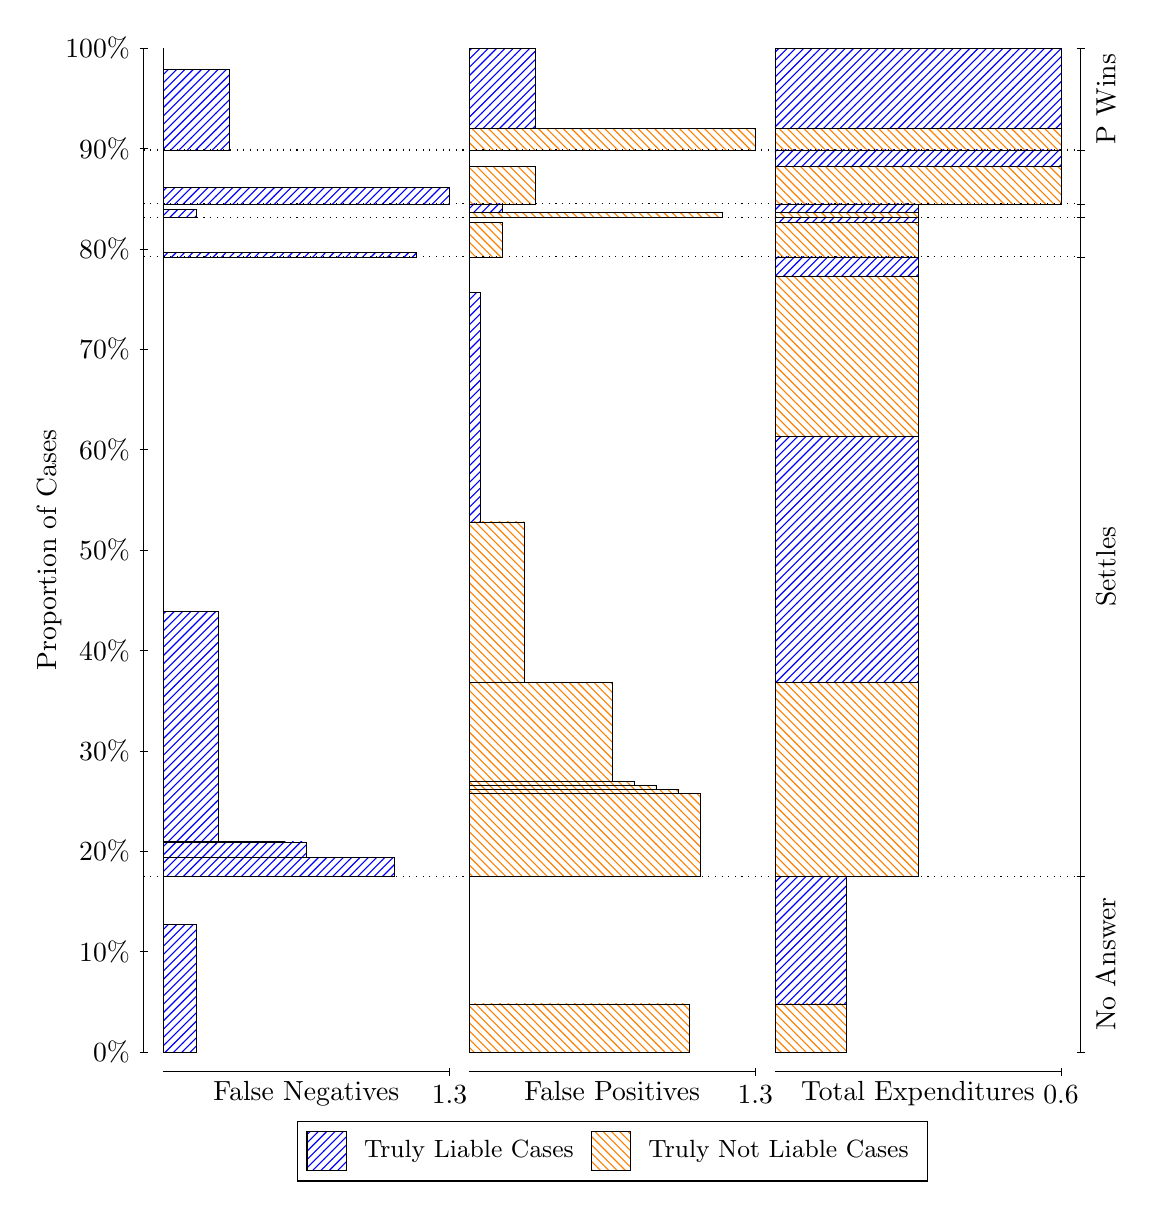
\begin{tikzpicture}
\draw[black, very thin] (1.5,1.75) -- (1.5,14.5);
\node[rotate=90, anchor=center] at (0.3, 8.125) {Proportion of Cases};
\draw[black, very thin] (1.45,1.75) -- (1.55,1.75);
\node[anchor=east] at (1.45, 1.75) {0\%};
\draw[black, very thin] (1.45,3.025) -- (1.55,3.025);
\node[anchor=east] at (1.45, 3.025) {10\%};
\draw[black, very thin] (1.45,4.3) -- (1.55,4.3);
\node[anchor=east] at (1.45, 4.3) {20\%};
\draw[black, very thin] (1.45,5.575) -- (1.55,5.575);
\node[anchor=east] at (1.45, 5.575) {30\%};
\draw[black, very thin] (1.45,6.85) -- (1.55,6.85);
\node[anchor=east] at (1.45, 6.85) {40\%};
\draw[black, very thin] (1.45,8.125) -- (1.55,8.125);
\node[anchor=east] at (1.45, 8.125) {50\%};
\draw[black, very thin] (1.45,9.4) -- (1.55,9.4);
\node[anchor=east] at (1.45, 9.4) {60\%};
\draw[black, very thin] (1.45,10.675) -- (1.55,10.675);
\node[anchor=east] at (1.45, 10.675) {70\%};
\draw[black, very thin] (1.45,11.95) -- (1.55,11.95);
\node[anchor=east] at (1.45, 11.95) {80\%};
\draw[black, very thin] (1.45,13.225) -- (1.55,13.225);
\node[anchor=east] at (1.45, 13.225) {90\%};
\draw[black, very thin] (1.45,14.5) -- (1.55,14.5);
\node[anchor=east] at (1.45, 14.5) {100\%};

\draw[black, very thin] (13.4,1.75) -- (13.4,14.5);
\draw[black, very thin] (13.35,1.75) -- (13.45,1.75);
\node[anchor=west] at (13.35, 1.75) {};
\draw[black, very thin] (13.35,3.9791) -- (13.45,3.9791);
\node[anchor=west] at (13.35, 3.9791) {};
\draw[black, very thin] (13.35,11.847) -- (13.45,11.847);
\node[anchor=west] at (13.35, 11.847) {};
\draw[black, very thin] (13.35,12.349) -- (13.45,12.349);
\node[anchor=west] at (13.35, 12.349) {};
\draw[black, very thin] (13.35,12.52) -- (13.45,12.52);
\node[anchor=west] at (13.35, 12.52) {};
\draw[black, very thin] (13.35,13.205) -- (13.45,13.205);
\node[anchor=west] at (13.35, 13.205) {};
\draw[black, very thin] (13.35,14.5) -- (13.45,14.5);
\node[anchor=west] at (13.35, 14.5) {};

\draw[black, very thin, pattern color=blue, pattern=north east lines] (1.75,1.75) rectangle (2.1692,3.3673);
\draw[black, very thin, pattern color=orange, pattern=north west lines] (1.75,3.3673) rectangle (1.75,3.9791);
\draw[black, very thin, pattern color=blue, pattern=north east lines] (1.75,3.9791) rectangle (4.6846,4.2196);
\draw[black, very thin, pattern color=blue, pattern=north east lines] (1.75,4.2196) rectangle (3.5667,4.4181);
\draw[black, very thin, pattern color=blue, pattern=north east lines] (1.75,4.4181) rectangle (3.2872,4.4214);
\draw[black, very thin, pattern color=blue, pattern=north east lines] (1.75,4.4214) rectangle (3.0077,4.4249);
\draw[black, very thin, pattern color=blue, pattern=north east lines] (1.75,4.4249) rectangle (2.7282,4.4284);
\draw[black, very thin, pattern color=blue, pattern=north east lines] (1.75,4.4284) rectangle (2.4487,7.3425);
\draw[black, very thin, pattern color=orange, pattern=north west lines] (1.75,7.3425) rectangle (1.75,11.847);
\draw[black, very thin, pattern color=blue, pattern=north east lines] (1.75,11.847) rectangle (4.9641,11.906);
\draw[black, very thin, pattern color=orange, pattern=north west lines] (1.75,11.906) rectangle (1.75,12.349);
\draw[black, very thin, pattern color=blue, pattern=north east lines] (1.75,12.349) rectangle (2.1692,12.453);
\draw[black, very thin, pattern color=orange, pattern=north west lines] (1.75,12.453) rectangle (1.75,12.52);
\draw[black, very thin, pattern color=blue, pattern=north east lines] (1.75,12.52) rectangle (5.3833,12.727);
\draw[black, very thin, pattern color=orange, pattern=north west lines] (1.75,12.727) rectangle (1.75,13.205);
\draw[black, very thin, pattern color=blue, pattern=north east lines] (1.75,13.205) rectangle (2.5885,14.229);
\draw[black, very thin, pattern color=orange, pattern=north west lines] (1.75,14.229) rectangle (1.75,14.5);
\draw[black, very thin, pattern color=orange, pattern=north west lines] (5.6333,1.75) rectangle (8.4282,2.3618);
\draw[black, very thin, pattern color=blue, pattern=north east lines] (5.6333,2.3618) rectangle (5.6333,3.9791);
\draw[black, very thin, pattern color=orange, pattern=north west lines] (5.6333,3.9791) rectangle (8.5679,5.0318);
\draw[black, very thin, pattern color=orange, pattern=north west lines] (5.6333,5.0318) rectangle (8.2885,5.0842);
\draw[black, very thin, pattern color=orange, pattern=north west lines] (5.6333,5.0842) rectangle (8.009,5.1354);
\draw[black, very thin, pattern color=orange, pattern=north west lines] (5.6333,5.1354) rectangle (7.7295,5.1857);
\draw[black, very thin, pattern color=orange, pattern=north west lines] (5.6333,5.1857) rectangle (7.45,6.4415);
\draw[black, very thin, pattern color=orange, pattern=north west lines] (5.6333,6.4415) rectangle (6.3321,8.4832);
\draw[black, very thin, pattern color=blue, pattern=north east lines] (5.6333,8.4832) rectangle (5.7731,11.397);
\draw[black, very thin, pattern color=blue, pattern=north east lines] (5.6333,11.397) rectangle (5.6333,11.847);
\draw[black, very thin, pattern color=orange, pattern=north west lines] (5.6333,11.847) rectangle (6.0526,12.29);
\draw[black, very thin, pattern color=blue, pattern=north east lines] (5.6333,12.29) rectangle (5.6333,12.349);
\draw[black, very thin, pattern color=orange, pattern=north west lines] (5.6333,12.349) rectangle (8.8474,12.416);
\draw[black, very thin, pattern color=blue, pattern=north east lines] (5.6333,12.416) rectangle (6.0526,12.52);
\draw[black, very thin, pattern color=orange, pattern=north west lines] (5.6333,12.52) rectangle (6.4718,12.998);
\draw[black, very thin, pattern color=blue, pattern=north east lines] (5.6333,12.998) rectangle (5.6333,13.205);
\draw[black, very thin, pattern color=orange, pattern=north west lines] (5.6333,13.205) rectangle (9.2667,13.477);
\draw[black, very thin, pattern color=blue, pattern=north east lines] (5.6333,13.477) rectangle (6.4718,14.5);
\draw[black, very thin, pattern color=orange, pattern=north west lines] (9.5167,1.75) rectangle (10.425,2.3618);
\draw[black, very thin, pattern color=blue, pattern=north east lines] (9.5167,2.3618) rectangle (10.425,3.9791);
\draw[black, very thin, pattern color=orange, pattern=north west lines] (9.5167,3.9791) rectangle (11.333,6.4415);
\draw[black, very thin, pattern color=blue, pattern=north east lines] (9.5167,6.4415) rectangle (11.333,9.5644);
\draw[black, very thin, pattern color=orange, pattern=north west lines] (9.5167,9.5644) rectangle (11.333,11.606);
\draw[black, very thin, pattern color=blue, pattern=north east lines] (9.5167,11.606) rectangle (11.333,11.847);
\draw[black, very thin, pattern color=orange, pattern=north west lines] (9.5167,11.847) rectangle (11.333,12.29);
\draw[black, very thin, pattern color=blue, pattern=north east lines] (9.5167,12.29) rectangle (11.333,12.349);
\draw[black, very thin, pattern color=orange, pattern=north west lines] (9.5167,12.349) rectangle (11.333,12.416);
\draw[black, very thin, pattern color=blue, pattern=north east lines] (9.5167,12.416) rectangle (11.333,12.52);
\draw[black, very thin, pattern color=orange, pattern=north west lines] (9.5167,12.52) rectangle (13.15,12.998);
\draw[black, very thin, pattern color=blue, pattern=north east lines] (9.5167,12.998) rectangle (13.15,13.205);
\draw[black, very thin, pattern color=orange, pattern=north west lines] (9.5167,13.205) rectangle (13.15,13.477);
\draw[black, very thin, pattern color=blue, pattern=north east lines] (9.5167,13.477) rectangle (13.15,14.5);
\draw[black, dotted] (1.5,3.9791) -- (13.4,3.9791);
\draw[black, dotted] (1.5,11.847) -- (13.4,11.847);
\draw[black, dotted] (1.5,12.349) -- (13.4,12.349);
\draw[black, dotted] (1.5,12.52) -- (13.4,12.52);
\draw[black, dotted] (1.5,13.205) -- (13.4,13.205);
\draw[black, very thin] (1.75,1.5) -- (5.3833,1.5);
\node[anchor=north] at (3.5667, 1.5) {False Negatives};
\draw[black, very thin] (5.3833,1.45) -- (5.3833,1.55);
\node[anchor=north] at (5.3833, 1.45) {1.3};

\draw[black, very thin] (5.6333,1.5) -- (9.2667,1.5);
\node[anchor=north] at (7.45, 1.5) {False Positives};
\draw[black, very thin] (9.2667,1.45) -- (9.2667,1.55);
\node[anchor=north] at (9.2667, 1.45) {1.3};

\draw[black, very thin] (9.5167,1.5) -- (13.15,1.5);
\node[anchor=north] at (11.333, 1.5) {Total Expenditures};
\draw[black, very thin] (13.15,1.45) -- (13.15,1.55);
\node[anchor=north] at (13.15, 1.45) {0.6};

\node[black, centered, rotate=90] at (13.72, 2.8645) {No Answer};
\node[black, centered, rotate=90] at (13.72, 7.9129) {Settles};



\node[black, centered, rotate=90] at (13.72, 13.853) {P Wins};

\draw (7.449999999999999,1.5) node[draw=none] (baseCoordinate) {};
\begin{scope}[align=center]
        \matrix[scale=0.5, draw=black, below=0.5cm of baseCoordinate, nodes={draw}, column sep=0.1cm]{
            \node[rectangle, draw, minimum width=0.5cm, minimum height=0.5cm, pattern=north east lines, pattern color=blue] {}; &
            \node[draw=none, font=\small] (B) {Truly Liable Cases}; &
            \node[rectangle, draw, minimum width=0.5cm, minimum height=0.5cm, pattern=north west lines, pattern color=orange] {}; &
            \node[draw=none, font=\small] (B) {Truly Not Liable Cases}; \\
            };
\end{scope}

\end{tikzpicture}
\end{document}